% ===============================
%          Chapter 1B.4
%       The Mammalian Heart
%     Created by Michael Tang
%           2025.01.12
% ===============================

\subsubsection{1B.4 The Mammalian Heart}
\paragraph{Structure of the Heart}
\begin{itemize}
    \item[1.] \textbf{General Description:}
    \begin{itemize}
        \item The heart is a \underline{four-chambered organ} (四腔器官) located in the \underline{thorax} (胸腔).
        \item Functions as a double pump to circulate oxygenated and deoxygenated blood.
        \item Composed of \underline{cardiac muscle} (心肌, specialized for continuous contraction without \underline{fatigue}
        疲倦).
    \end{itemize}
    \item[2.] \textbf{Chambers:}
    \begin{itemize}
        \item \textbf{\underline{Right Atrium} (右心房):} Recieves deoxygenated blood from the body via the \underline{vena cava}
        (腔静脉).
        \item \textbf{\underline{Right Ventricle} (右心室):} Pumps deoxygenated blood to the lungs via the \underline{pulmonary
        artery} (肺动脉).
        \item \textbf{\underline{Left Atrium} (左心房):} Recieves oxygenated blood from the lungs via the \underline{pulmonary
        vein} (肺静脉).
        \item \textbf{\underline{Left Ventricle} (左心室):} Pumps oxygenated blood to the body via the \underline{aorta} (主动脉).
        It has thicker walls than the right ventricle to withstand higher pressure.
    \end{itemize}
    \item[3.] \textbf{Key Structure:}
    \begin{itemize}
        \item \textbf{\underline{Septum} (隔膜):} Thick muscular wall seperating the left and right sides of the heart.
        \item \textbf{\underline{Valves} (瓣膜):} Prevent backflow of blood:
        \begin{itemize}
            \item \textbf{\underline{Tricuspid Valve} (三尖瓣):} Between the right atrium and ventricle.
            \item \textbf{\underline{Bicuspid (Mitral) Valve} (二尖瓣):} Between the left atrium and ventricle.
            \item \textbf{\underline{Semilunar Valves} (半月瓣):} At the exit of the pulmonary artery and aorta.
        \end{itemize}
        \item \textbf{\underline{Tendineae Cords} (腱索 Chordae Tendineae):} Prevent valves from inverting under pressure.
    \end{itemize}
    \item[4.] \textbf{\underline{Coronary Circulation} (冠状循环):}
    \begin{itemize}
        \item The heart muscle is supplied with oxygenand nutrients by the \underline{coronary arteries} (冠状动脉).
        \item Rich in \underline{myoglobin} (肌红蛋白), a \underline{respiratory pigment} (呼吸色素) with a higher oxygen
        \underline{affinity} (亲和力) than hemoglobin.
    \end{itemize}
    \begin{figure}[H]
        \centering
        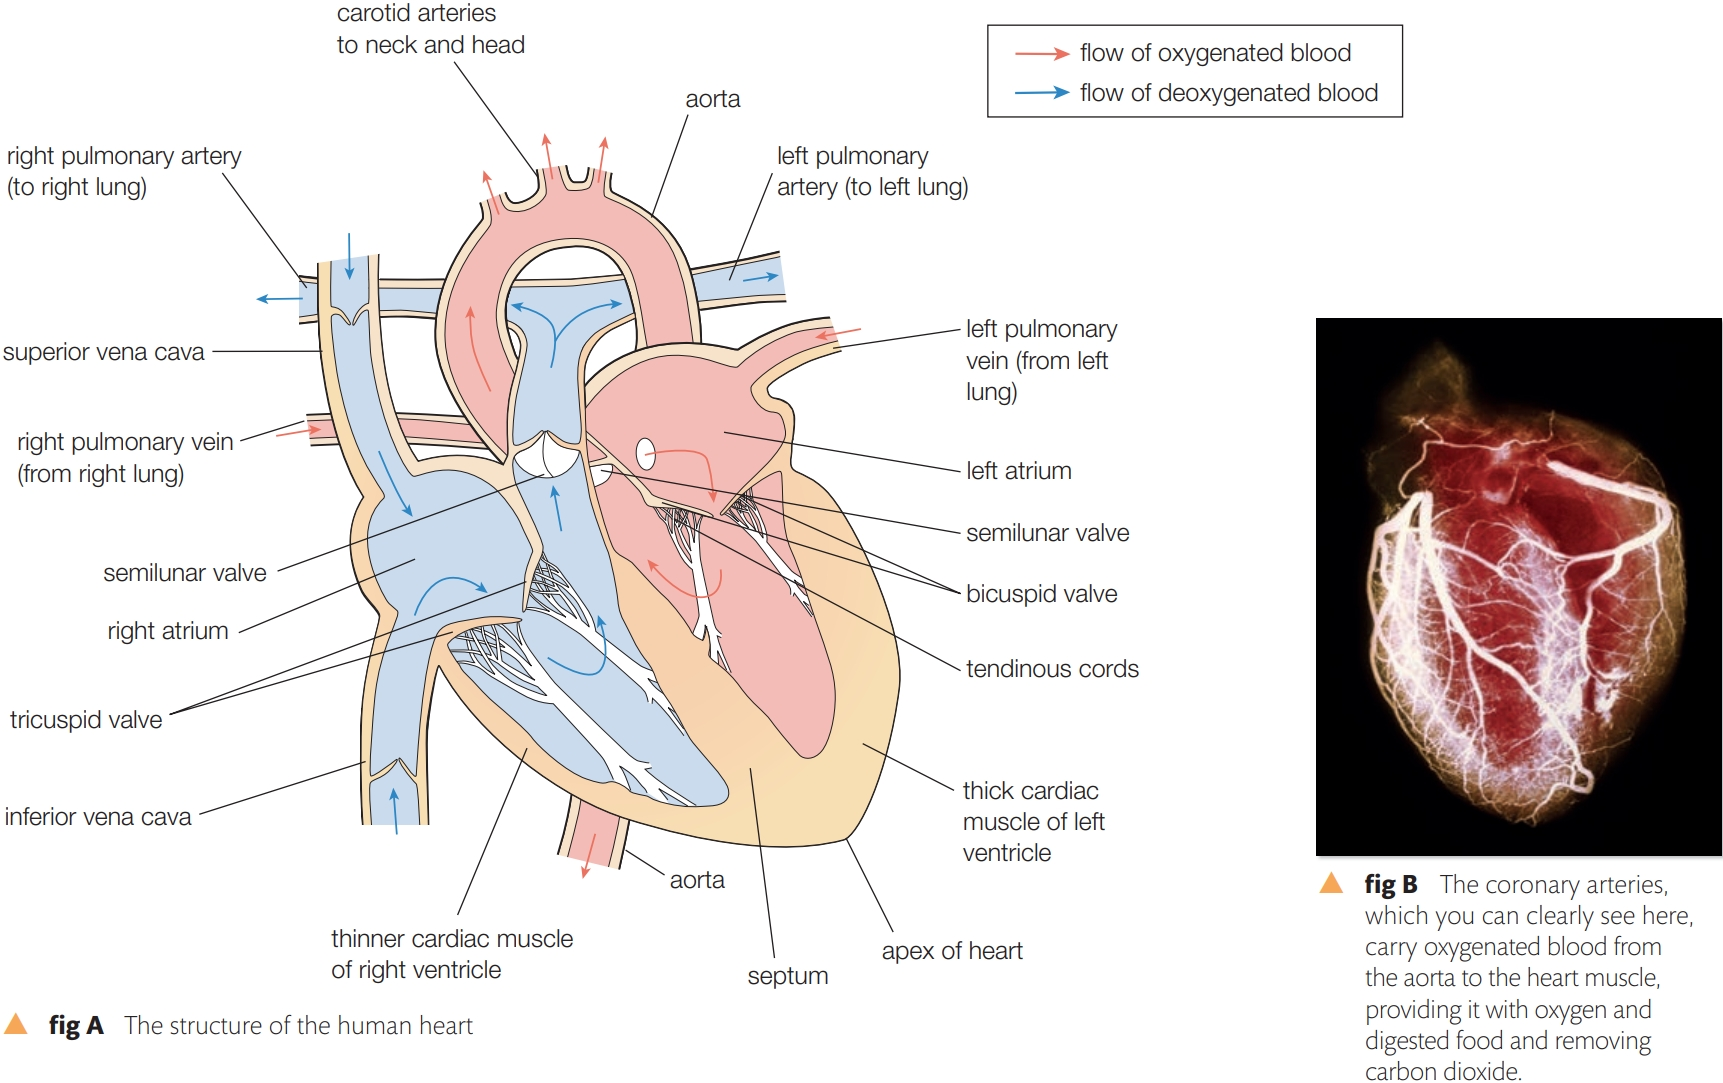
\includegraphics[scale=0.25]{Biology/1B/Images/1B-4-1.png}
    \end{figure}
\end{itemize}

\paragraph{Action of the Heart}
\begin{itemize}
    \item \textbf{Blood Flow Sequence:}
    \begin{itemize}
        \item[1.] \textbf{Deoxygenated Blood:}
        \begin{itemize}
            \item Enters the right atrium via the \underline{vena cava} (腔静脉).
            \item Flows into the left ventricle through the \underline{tricuspid valve} (三尖瓣).
            \item Is pumped to the body through the aorta.
        \end{itemize}
        \item[2.] \textbf{Oxygenated Blood:}
        \begin{itemize}
            \item Returns from the lungs to the left atrium via the \underline{pulmonary vein} (肺静脉).
            \item Flows into the left ventricle through the \underline{bicuspid valve} (二尖瓣).
            \item Is pumped to the body through the aorta.
        \end{itemize}
    \end{itemize}
    \item \textbf{Valve Function:}
    \begin{itemize}
        \item Valves open and close due to pressure difference to ensure \underline{unidirectional flow} (单向流动).
        \item Semilunar valves prevent backflow from arteries to ventricles.
        \item \underline{Atrioventricular valves} (房室瓣) prevent backflow from ventricles to atria.
    \end{itemize}
    \item \textbf{Pressure Adaptation:}
    \begin{itemize}
        \item The left ventricle has a thicker muscular wall to pump blood at higher pressure to the \underline{systemic circuit}
        (体循环).
        \item The right ventricle pumps blood at lower pressure to the lungs to avoid damaging the delicate capillaries.
    \end{itemize}
\end{itemize}

\paragraph{The Cardiac Cycle}
\begin{itemize}
    \item \textbf{Phases:}
    \begin{itemize}
        \item \textbf{\underline{Atrial Systole} (心房收缩):} Atria contract, forcing blood into the ventricles.
        \item \textbf{\underline{Ventricular Systole} (心室收缩):} Ventricles contract, pumping blood to the lungs and body.
        \item \textbf{\underline{Diastole} (舒张期):} Both atria and ventricles relax, allowing chambers to fill with blood.
    \end{itemize}
    \item \textbf{Heartbeat Sounds:}
    \begin{itemize}
        \item \textbf{\underline{'Lub' Sound} (第一心音):} Closing of atrioventricular valves during ventricular systole.
        \item \textbf{\underline{'Dub' Sound} (第二心音):} Closing of semilunar valves during ventricular diastole.
    \end{itemize}
    \item \textbf{Cycle Duration:} Each cardiac cycle lasts approximately 0.8 seconds in humans:
    \begin{itemize}
        \item Atrial systole: 0.1 seconds.
        \item Ventricular systole: 0.3 seconds.
        \item Diastole: 0.4 seconds.
    \end{itemize}
    \begin{figure}[H]
        \centering
        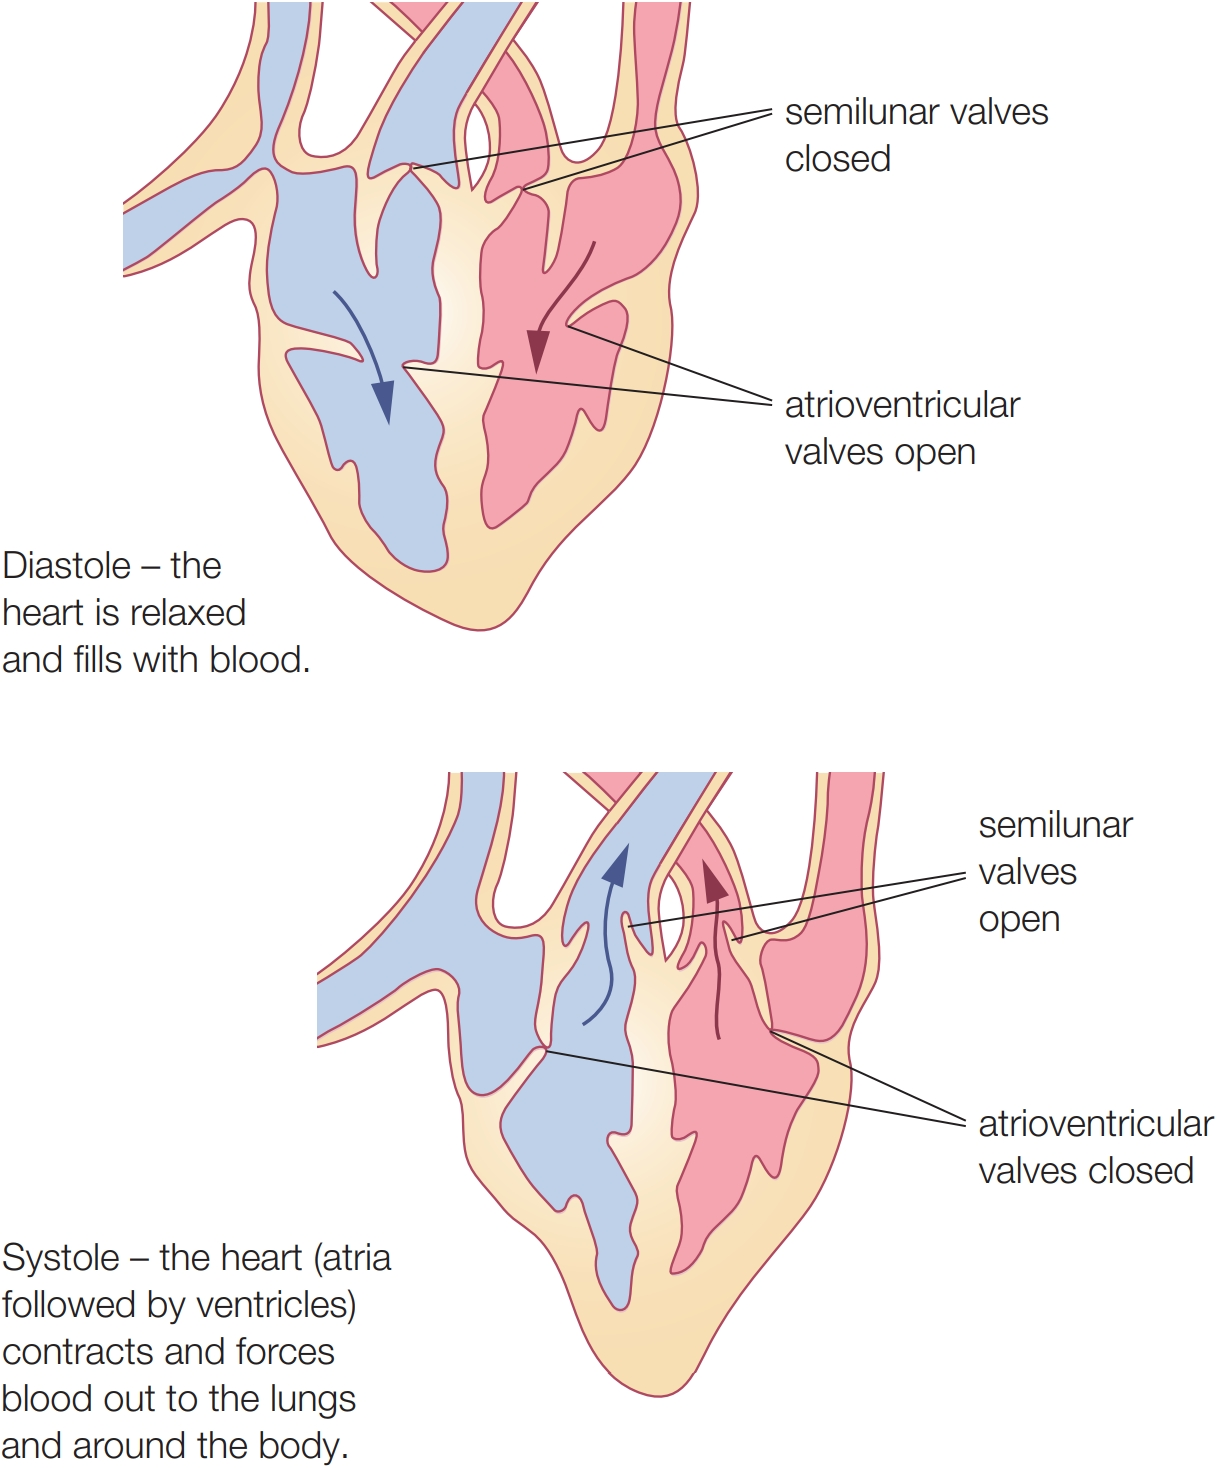
\includegraphics[scale=0.15]{Biology/1B/Images/1B-4-2.png}
        \caption{The cardiac cycle.}
    \end{figure}
\end{itemize}